\documentclass[uplatex,dvipdfmx,a4j,11pt]{jsreport}
\usepackage[utf8]{inputenc}
\usepackage[dvipdfmx]{graphicx,xcolor}
\usepackage{amsmath, amssymb, amsfonts, latexsym, mathtools}
\usepackage{amsthm}
\usepackage{url}
\usepackage{hyperref}
\usepackage{tcolorbox}
\tcbuselibrary{skins, breakable, theorems}
\usepackage{cleveref} %参照用
\usepackage{enumerate}
\usepackage{fancyhdr}
\usepackage{tikz}
\usepackage{pifont}
\usepackage{appendix}
\setcounter{tocdepth}{3}
\usepackage{perpage}
\MakePerPage{footnote}
\usepackage{wrapfig}
\usepackage{here}
\usepackage[hang,small,bf]{caption}
\usepackage[subrefformat=parens]{subcaption}

% 色の定義
\definecolor{mainblue}{RGB}{0,102,204}
\definecolor{lightblue}{RGB}{230,240,255}
\definecolor{darkgreen}{RGB}{0,128,0}
\definecolor{lightgreen}{RGB}{240,255,240}
\definecolor{orange}{RGB}{255,140,0}
\definecolor{lightorange}{RGB}{255,250,240}
\definecolor{purple}{RGB}{128,0,128}
\definecolor{lightpurple}{RGB}{250,240,255}
\definecolor{darkred}{RGB}{139,0,0}
\definecolor{lightgray}{RGB}{245,245,245}

% 定義ボックス
\newtcolorbox[auto counter, number within=chapter, crefname = {定義}{定義}]{definition}[4][]{
  enhanced,
  colback=lightblue,
  colframe=mainblue,
  colbacktitle=mainblue,
  fonttitle=\bfseries,
  coltitle=white,
  boxrule=1pt,
  arc=2mm,
  breakable,
  enhanced,
  title=定義~\if #4(#4)\else \thetcbcounter\fi~ #2,
  #1,
  label = def:#3
}

\newtcolorbox[auto counter, number within=chapter, crefname = {注意}{注意}]{remark}[4][]{
  enhanced,
  colback=lightgray,
  colframe=darkgreen,
  colbacktitle=darkgreen,
  fonttitle=\bfseries,
  coltitle=white,
  boxrule=1pt,
  arc=2mm,
  breakable,
  enhanced,
  title=注意~\if #4(#4)\else \thetcbcounter\fi~ #2,
  #1,
  label = rem:#3
}

\newtcolorbox[auto counter, number within=chapter, crefname = {余談}{余談}]{aside}[4][]{
  enhanced,
  colback=lightorange,
  colframe=orange,
  colbacktitle=orange,
  fonttitle=\bfseries,
  coltitle=white,
  boxrule=1pt,
  arc=2mm,
  breakable,
  title=余談~\if #4(#4)\else \thetcbcounter\fi~ #2,
  #1,
  label = aside:#3
}

% コマンド定義
\newcommand{\keyword}[1]{\textcolor{mainblue}{\textbf{#1}}}
\newcommand{\important}[1]{\textcolor{darkred}{\textbf{#1}}}
\newcommand{\highlight}[1]{\colorbox{yellow!30}{#1}}
\newcommand{\divergence}{\mathrm{div}\,}  %ダイバージェンス
\newcommand{\grad}{\mathrm{grad}\,}  %グラディエント
\newcommand{\rot}{\mathrm{rot}\,}  %ローテーション
\newcommand{\e}{\mathbf{e}} % 単位ベクトル
\newcommand{\diff}{\mathrm{d}} % 微分
\newcommand{\Diff}{\mathrm{D}} % 微分

\def\thefootnote{\fnsymbol{footnote}}

% ページスタイル
\pagestyle{fancy}
\fancyhf{}
% 「第N章. 章タイトル」形式で左上に表示
\renewcommand{\chaptermark}[1]{%
  \markboth{第\thechapter 章. #1}{}}
\fancyhead[L]{\leftmark}
\fancyhead[R]{\thepage}
\renewcommand{\headrulewidth}{0.4pt}

\hypersetup{
  hidelinks,
  bookmarksnumbered=true
}

% 式番号を (章).## 形式にする
\numberwithin{equation}{chapter}

% cleverefの日本語化
\crefname{figure}{図}{図}
\crefname{equation}{式}{式}
\crefname{table}{表}{表}
\crefname{chapter}{章}{章}
\crefname{section}{節}{節}

\begin{document}

\title{\Huge\textbf{空気力学の基礎(仮称)}}
\author{佐藤 空馬 (14期代空力班長)\footnotemark}
\date{\today}
\footnotetext{
\begin{tabular}{@{}l@{}l@{}}
GitHub: \qquad & \url{https://github.com/kuma003} (Univ. account) \\
  & \url{https://github.com/kuma-1220} (Personal account)
\end{tabular}
}
\maketitle

\tableofcontents

\chapter{初めに}
\section{基本用語の整理}
この章では,基本的な用語を整理する.
種々の詳細や導出については次章以降で述べるので,必要に応じて参照されたい.

\subsection{流体力学}
液体や気体 (総じて\keyword{流体}) の力学的性質を研究する学問を \keyword{流体力学} という.

\enskip

流体の流れは,その流れの様子により \keyword{層流} (Laminar flow) と \keyword{乱流} (Turbulent flow) に大別される.
その名の通り,層流はいわば整った流れであり,乱流は不規則な流れである.
より厳密には,流れの状態は \keyword{レイノルズ数} (Reynolds number) という無次元数により決定される.
これは,慣性力と粘性力の比を表すものであり,その定義は以下の通りである.
\begin{definition}{レイノルズ数$\textit{Re}$}{Reynolds}{}
   流体の慣性力と粘性力の比を表す無次元数.
    \begin{equation}
      \textit{Re} \equiv \frac{\text{慣性力}}{\text{粘性力}}
      = \frac{\rho UL}{\mu} = \frac{UL}{\nu}
    \end{equation}
  ただし,$\rho$は流体の密度,$U$は代表速度,$L$は代表長さ,$\mu$は粘性係数,$\nu$は動粘性係数である.
  ここで,代表速度・代表長さはそれぞれ対象とする系によって取り方が異なる (そのため,この値はあくまでも目安である).
\end{definition}
このレイノルズ数が小さい場合,粘性力が支配的であり,流れは層流となる.
一方で,レイノルズ数が大きい場合,慣性力が支配的であり,流体の各要素がめいめい自由に動こうとするため,流れは乱流となる.
一般的に,レイノルズ数が約2300以上であれば乱流となる.

\enskip

次に,支配方程式の話に移ろう.
定常(すなわち流れが時間的に変化しない)・非圧縮流れの場合,流体の運動は \keyword{ベルヌーイの定理} (Bernoulli's theorem) に従う.
以下にその定理を示す.
第二式からわかるように,本質的には\emph{流線上のエネルギー保存則}である.
\begin{definition}{ベルヌーイの定理}{Bernoulli}{}
   定常・非圧縮流れにおいて,流線上の任意の点で成り立つ関係式.
  以下のように,次元の異なる3通りの表現があるが,いずれも同じ内容を表している.
  \begin{align}
  	\text{圧力の次元}:      &\quad p + \frac{1}{2}\rho U^{2} + \rho g h = \mathrm{const.}\\
  	\text{エネルギーの次元}:&\quad \frac{p}{\rho} + \frac{1}{2} U^{2} + g h = \mathrm{const.}\\
  	\text{高さの次元}:      &\quad \frac{p}{\rho g} + \frac{U^{2}}{2g} + h = \mathrm{const.}
  \end{align}

  ただし,$p$は圧力,$\rho$は流体の密度,$U$は流体の速度,$g$は重力加速度,$h$は基準面からの高さである.

   補足として,一部の項には特別な名前が付けられている.
  第一式について,流体が持つ圧力$p$を特に\keyword{静圧},$\frac{1}{2}\rho U^{2}$を\keyword{動圧}という.
  また,第三式について,このような形で表される値を水頭(Water Head)と呼び,それぞれ
  $\frac{p}{\rho g}$を\keyword{圧力水頭},$\frac{U^{2}}{2g}$を\keyword{速度水頭},$h$を\keyword{位置水頭}という.
\end{definition}

例えば,流れの中に置かれた物体が受ける力を考えよう.
物体表面では流体の速度が0になる(このような点を \keyword{よどみ点}(Stagnation Point)という).
したがって,ベルヌーイの法則から動圧がすべて静圧に変換される.
これによって,流れの中に置かれた物体は,流れの方向に動圧$ \frac{1}{2}\rho U^{2} $を受けることになる.
このようによどみ点で受ける圧力を特に \keyword{よどみ圧} (Stagnation Pressure) という.

\enskip

より一般の系,すなわち非定常・圧縮流れ・粘性流れの場合,流体の運動は \keyword{ナビエ--ストークス方程式} (Navier--Stokes equations; NS eq.) に従う.
以下にその方程式を示す.
\begin{definition}{ナビエ--ストークス方程式}{NSE}{}
  ナビエ--ストークス方程式とは,流体の運動を記述するための偏微分方程式である.
  これらの方程式は,質量保存則,運動量保存則,エネルギー保存則を基に導かれる.
    \begin{equation}
    \frac{\partial \mathbf{u}}{\partial t} + (\mathbf{u} \cdot \nabla) \mathbf{u} = -\frac{1}{\rho} \nabla p + \nu \nabla^{2} \mathbf{u} + \mathbf{g}
    \end{equation}
  ただし,$\mathbf{u}$は流体の速度ベクトル,$p$は圧力,$\rho$は流体の密度,$\nu$は動粘性係数,$\mathbf{g}$は外力項である.

\end{definition}
詳細についてここでは踏み入らないが,非線形であるため解析的に解くことは困難であり,数値的に (すなわちコンピュータを用いて) 解くことが一般的である.

\subsection{空気力学}
空気中を飛翔する物体 (以下,飛翔体) には,その空気の流れに伴って様々な力が作用する.このような力の発生機構やその影響を研究する学問を\keyword{空気力学}という.
ここでは,基本的な用語を紹介し,詳細な導出については次節以降に述べる.

\enskip

まず,飛翔体に作用する力を整理しよう.
以下に示すように,飛翔体には流れ方向に\keyword{抗力} (Drag force) が,流れに垂直な方向に\keyword{揚力} (Lift force) が作用する (\cref{fig:drag_lift}).
一方で,これらの力を機軸方向とそれに垂直な方向にも分解することができる (\cref{fig:axial_normal}).
これら方向の力をそれぞれ \keyword{軸力} (Axial force) と \keyword{法線力} (Normal force) と呼ぶ.

\begin{figure}[H]
  \centering
  \begin{minipage}{\hsize}
    \centering
    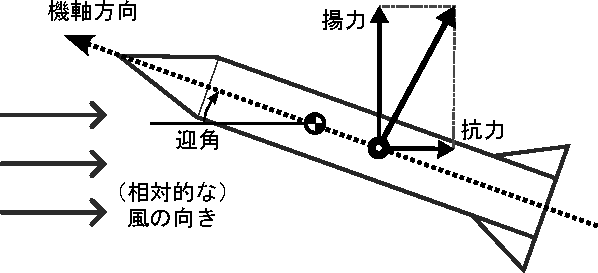
\includegraphics{aero/img/drag_lift.pdf}
    \subcaption{抗力と揚力.}
    \label{fig:drag_lift}
  \end{minipage}\\
  \begin{minipage}{\hsize}
    \centering
    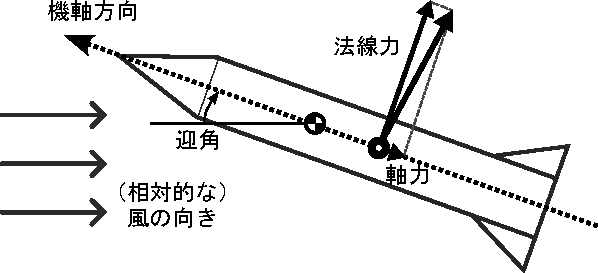
\includegraphics{aero/img/axial_normal.pdf}
    \subcaption{軸力と法線力.}
    \label{fig:axial_normal}
  \end{minipage}
  \caption{大気中を飛翔する物体に作用する力.}
\end{figure}


先に述べたように,流れ場に置かれた物体表面にはよどみ圧$\frac{1}{2}\rho U^{2}$が作用する.
よって,物体表面全体にわたってこの表面にかかる圧力を積分すると,物体に作用する力を求めることができる.
物体表面全体にわたってこの圧力が作用すると考えると
おおよそ動圧$\frac{1}{2}\rho U^{2}$に比例した大きさの力が物体に作用すると考えられる
\footnote{
  無論,厳密には不適当な議論である.ベルヌーイの定理を立脚点に計算すると,圧力の表面積分は0になることが知られている.
  これを \keyword{ダランベールのパラドクス}(D'Alembert's paradox)という.
  このパラドクスを解決するためには粘性や圧縮性の影響を取り入れたナビエ--ストークス方程式を解く必要がある.
}.

そこで,これら値を無次元化することを考えよう.
先の議論から,物体に作用する力は動圧$\frac{1}{2}\rho U^{2}$に比例すると考えられ,また抗力なら断面積にも比例すると考えられる.
したがって,これらの値で除して無次元化することで,流速や飛翔体の大きさが異なる場合でも,力の大きさを比較することができる.
\begin{definition}{力の無次元化 1}{}{}
   無次元化とは,物理量を無次元数で表現することであり,これによってスケールの物理現象を比較することが可能になる.
  以下に,抗力と法線力を無次元化した,\keyword{抗力係数} (Drag force coefficient) $C_{D}$ と\keyword{法線力係数} (Normal force coefficient) $C_{N}$ を示す.
    \begin{equation}
      C_{D} \equiv \frac{D}{\frac{1}{2}\rho U^{2}A}, \quad C_{N} \equiv \frac{N}{\frac{1}{2}\rho U^{2}A}
    \end{equation}
  ただし,$D$は抗力,$N$は法線力,$\rho$は流体の密度,$U$は流体の速度,$A$は物体の代表面積である.
  なお,これらの定義は軸力や揚力についても同様に適用できる.
  また,代表面積は物体の正面投影面積 (つまり断面積) を用いることが多いが,例えば翼の揚力を解析する場合などには動圧と翼面積で無次元化することもある.
\end{definition}

また,揚力であれば物体の姿勢にも依存するであろうと考えられる.
実際には,\keyword{迎角・迎え角} (Angle of Attack; AoA) という,機軸と流れ方向がなす角度に比例することが知られている.
また,低迎角であれば法線力と揚力は一致するため,法線力係数も迎角に比例すると考えられる.
そこで,次のように法線力係数を迎角で除してみよう:
\begin{definition}{力の無次元化 2}{}{}
   法線力係数を迎角で除して無次元化することで,以下のような \keyword{法線力係数傾斜} (Normal force coefficient slope) $C_{N\alpha}$ を定義することができる.
    \begin{equation}
      C_{N\alpha} \equiv \frac{C_{N}}{\alpha}
    \end{equation}
  ただし,$\alpha$は迎角 [単位: rad] であるため単位は $[\mathrm{rad}^{-1}]$ となるが,ラジアンは無次元であるため結局は無次元数である.
  ここで傾斜というのは,低迎角であれば法線力係数が迎角に比例することに由来する (i.e. $C_N = C_{N\alpha} \alpha$) .
  % 勿論,非低迎角の場合には迎角の2次以上の項も現れるが,ロケットの場合は低迎角の場合が多いため,あまり問題にならない.
\end{definition}

\enskip

次に,モーメントについても考えよう.
以下にモーメントの無次元化を紹介する.ただし,実用上この定義式を用いることは少ない.
\begin{definition}{モーメントの無次元化}{}{}
  モーメントの無次元化は以下のように定義される.
    \begin{equation}
      C_M \equiv \frac{M}{\frac{1}{2}\rho U^{2}A L}
    \end{equation}
  ただし,$M$はモーメント,$L$は物体の代表長さである.
\end{definition}

ロケットにおいては,フィンの不整合によるモーメントやエンジンの燃焼によるモーメント
\footnote{これを \emph{ジェットダンピングモーメント} (Jet Damping Moment) という.これは燃焼・排気されるガスがロケットから持ち去る角運動量に起因する.},
その他さまざまな要因でモーメントが発生するが,最も顕著なのは\emph{法線力によるモーメント}である.
ここでは法線力によるモーメントについて議論する.

このモーメントを議論する上で重要なのは,力の作用点である.
これを,\keyword{圧力中心} (Center of Pressure; CP) と呼ぶ.
動力学の議論から,任意の物体は重心を通る軸を中心に回転することがわかっている.
したがって,圧力中心と重心の位置関係がモーメントの発生に重要な役割を果たす.
\begin{definition}{圧力中心}{CP}{}
   圧力中心とは,物体に作用する法線力の合力の作用点のことである:
    \begin{equation}
      C_\mathrm{P} \equiv \frac{\int N(x)x\,\diff x}{\int N(x)\,\diff x}
    \end{equation}
  ここで,積分は機軸方向にわたって行い,$N(x)$は位置$x$における法線力分布である.

   各コンポーネント$i$ (e.g. ノーズ,ボディ,フィン,etc.) の圧力中心を$C_{\mathrm{P}i}$,法線力を$N_i$とすると,以下のようにも表現できる.
  \begin{equation}
    C_\mathrm{P} = \frac{\sum_i N_i C_{\mathrm{P}i}}{\sum_i N_i}
  \end{equation}
\end{definition}

\begin{remark}{重心}{CG}{}
   念のため,重心の定義を以下に示す.圧力中心の定義と対称的なのがわかる.
    \begin{equation}
      C_\mathrm{G} \equiv \frac{\int \lambda(x)x\,\diff x}{\int \lambda(x)\,\diff x}
    \end{equation}
  ここで,積分は機軸方向にわたって行い,$\lambda(x)$は位置$x$における線密度分布である.
\end{remark}

ロケットの安定性を議論するときに用いられる安定比は,以下のように定義される.
\begin{definition}{安定比}{}{}
  ロケットにおける安定比とは,圧力中心と重心の位置関係を示す指標であり,以下のように定義される.
    \begin{equation}
      \text{Stability Margin} \equiv \frac{C_\mathrm{P} - C_\mathrm{G}}{L}
    \end{equation}
  ここで,$L$は物体の機体長である.また,圧力中心・重心ともに先頭からの長さを表している.
\end{definition}
図を描けば明らかなように,安定であるためには,圧力中心が重心よりも後方に位置しなければならない.
すなわち,安定比は正である必要がある.
一方で,過大な安定比は,\emph{風見効果}というロケットが風上に向かう現象を強くし,横風に対して不安定になる.
従って,安定比は10-20\%程度が望ましいとされる.

\enskip

また,増大するモーメントに対してそれを減衰させる方向にモーメントがはたらく.
これを\keyword{ダンピングモーメント} (Damping moment) という.
これまでの議論はすべて静的なものを仮定していたが,これは動的な効果であり,ロケットの過去の運動履歴に依存する
\footnote{これはナビエ--ストークス方程式の非線形性に起因する.} .

ここでは,簡単に一般の減衰モーメント係数の定義と,
ロケットにおけるピッチ・ヨー減衰モーメント係数,ロール減衰モーメント係数について以下に示す.
詳細については本稿では立ち入らないため,必要に応じて詳細をまとめた拙稿『減衰モーメント係数について』を参照されたい.
\begin{definition}{減衰モーメント係数}{}{}
   一般に,減衰モーメント係数は以下によって定義される:
  \begin{equation}
  C_{m\dot{\theta}} = \frac{4}{\rho v^2 S L}\frac{v}{L}\frac{\partial M}{\partial\dot{\theta}} \label{fte_def}
\end{equation}
特に,ロケットにおけるピッチ・ヨー減衰モーメント係数$C_{mq}$, ロール減衰モーメント係数$C_{mp}$は,
\begin{gather}
  C_{mq} = - 4 \sum_i \left(\frac{C_{n\alpha i}}{2}\right)\left(\frac{C_{pi} - C_{g}}{L}\right)^2,\\
  C_{mp} = - 8 \times \cfrac{\left(\mathrm{span} + d/2\right)^4}{\pi L^2 \cfrac{\pi d^2}{4}}.
\end{gather}
\end{definition}

\enskip

また,ナビエ--ストークス方程式の非線形性に起因して,\keyword{フラッタリング} (Flutter) といった空力的に不安定な現象が発生することがある.
これは主に翼に関する現象であり,窓ガラスがカタカタと震えるように,翼が振動する現象である.
特定の速度以上では,この振動が増幅され,最終的に翼の破壊に至ることがある.

\subsection{数値解析}
先に述べたように,ナビエ--ストークス方程式は非線形であるため解析的に解くことは困難であり,数値的に解くことが一般的である.
この手法を \keyword{数値流体力学} (Computational Fluid Dynamics; CFD) という.
\cref{def:NSE}で示したように,ナビエ--ストークス方程式は偏微分方程式で記述される.
微分とは,つまるところ二点間の距離や時間間隔を極限まで小さくしたときの変化率を表すものである.
従って,空間を細かく区切ることで,この微分を差分で近似することができる.
この区切られた空間を \keyword{メッシュ} (Mesh) と呼ぶ.

\enskip

飛行シミュレーションについても同様である.
ロケットの飛行シミュレーションでは,運動をモデル化して得られる運動方程式から,ロケットの運動を数値的に解くことで,飛行軌道を予測する.
その詳細については後の章で詳述する.


\chapter{流体力学}

このセクションでは,流体力学の基礎についてナビエストークス方程式をまず初めに導出し,
その後ベルヌーイの定理やポテンシャル流について説明する.
歴史的な順番からはベルヌーイの定理を先に説明するべきかもしれないが,ここでは理論に重きを置くため,ナビエ--ストークス方程式を先に説明することに注意されたい.

\section{ナビエ--ストークス方程式}
\subsection{ガウスの方法とラグランジュの方法}
本題に入る前に,流体力学における二つの主要な見方である,オイラーの方法とラグランジュの方法について説明する.

\begin{definition}{オイラーの方法}{}{}
   \keyword{オイラーの方法}とは,空間のある固定された一点に注目し,その点を流体が通過していく様子を観察する方法である.
  ある物理量$A$を指定するには$A(x,y,z,t)$または,$A(\mathbf{r},t)$と表現すればよい.
\end{definition}

\begin{definition}{ラグランジュの方法}{}{}
   \keyword{ラグランジュの方法}とは,ある特定の微小流体要素
  \footnote{
  勿論,個々の原子・分子はブラウン運動するため,流体要素としてこれらをイメージするのは不適当である.
  それよりも大きい仮想的な微小要素をイメージするのが妥当である.
  }
  に注目し,その流体要素が時間とともにどのように変化するかを観察する方法である.
  ラグランジュの方法において
  ある物理量$A$を指定するには$A_{\mathbf{r}}(t)$と表現すればよい.
  ただしここで添字の位置ベクトル$\mathbf{r}$は,その流体要素が初めにその位置$\mathbf{r}$に存在したという程度の意味である.
\end{definition}

ここでラグランジュの方法に関連して,流線・流跡線・流脈線それぞれの違いを以下に説明する.
\begin{definition}{流線・流跡線・流脈線}{}{}
   流線・流跡線・流脈線の違いを以下にまとめる.
  \begin{center}
  \begin{tabular}{cl}
    \hline
    用語 & 定義 \\
    \hline
    流線 & 各時刻において,流体の速度ベクトルが接線となる曲線 \\
    流跡線 & 流体のある点を通過した粒子の軌跡 \\
    流脈線 & ある点を通過した粒子をつないだ曲線 \\
    \hline
  \end{tabular}
  \end{center}
  これらは一般には異なるが,定常流においては一致する.
\end{definition}
例えば風洞実験の写真などでよく見られる煙の流れは,流線ではなくて流脈線を可視化したものであると言える
\footnote{ただし,風洞実験で煙を用いて流れを見る場合には定常的な場合が殆どであるため,流線と言っても差し支えない.}.

\enskip

さて,流跡上でのある流体粒子が微小時間で移動する間に,その物理量がどのように変化するかを考えてみよう.
これはラグランジュ的な方法における時間微分に相当する.

微小時間変化を$\Delta t$とすると,変位は三次元座標系において,
\begin{equation*}
  \Delta \mathbf{r} = \mathbf{u} \Delta t
\end{equation*}
と表される.
したがって,流跡上での微分はテーラー展開を用いると,
\begin{align*}
  \lim_{\Delta t \to 0} \frac{A_\mathbf{r}(t + \Delta t) - A_\mathbf{r}(t)}{\Delta t}
  &= \lim_{\Delta t \to 0} \frac{A(\mathbf{r} + \mathbf{u} \Delta t, t + \Delta t) - A(\mathbf{r}, t)}{\Delta t}\\
  &= \lim_{\Delta t \to 0} \frac{1}{\Delta t}\left((\nabla A(\mathbf{r}, t))\cdot \mathbf{u}\Delta t  + \frac{\partial A(\mathbf{r}, t)}{\partial t}\Delta t\right)\\
  &= \left(\mathbf{u}\cdot \nabla + \frac{\partial }{\partial t}\right) A(\mathbf{r}, t)
\end{align*}
となる.この微分を流体要素 (物質) に注目した微分であるから,物質微分と呼び,以下のように表記する:
\begin{equation*}
  \frac{\Diff}{\Diff t} A(\mathbf{r}, t) = \left(\mathbf{u}\cdot \nabla + \frac{\partial }{\partial t}\right) A(\mathbf{r}, t)
\end{equation*}

\begin{definition}{物質微分}{}{}
   \keyword{物質微分} (Material derivative) とは,ラグランジュの方法に基づいた流体要素からみた時間微分であり,以下のように表される.
    \begin{equation}
      \frac{\Diff}{\Diff t} = \frac{\partial }{\partial t} + \mathbf{u}\cdot \nabla
    \end{equation}
\end{definition}

\subsection{ナビエ--ストークス方程式の簡単な導出}

まず始めに,粘性が作用しない流体 (\keyword{完全流体} (Ideal fluid)) から考えよう.

微小流体要素を,その体積が$\Delta x \Delta y \Delta z = \Delta V$なる微小立方体とする.
\cref{fig:pressure_differential}を参考に,このとき圧力によって$x$方向にかかる力を考察しよう.

\begin{figure}[h]
  \centering
  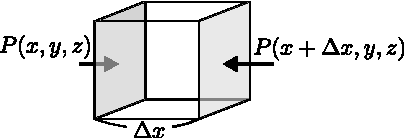
\includegraphics{aero/img/pressure_differential.pdf}
  \caption{$x$方向の圧力差.}
  \label{fig:pressure_differential}
\end{figure}

図中のように,微小立方体の左右からかかる圧力差が物体の$x$方向にかかる力に相当する.
ここで,圧力はすべて\cref{fig:pressure_differential}に示すように,すべて立方体に入る向きに作用することに注意しよう.
このとき,微小立方体の圧力差による力は次のように表される.
  \begin{equation}
    F_x = -\left(P(x + \Delta x, y, z) - P(x, y, z)\right) \Delta y \Delta z.
  \end{equation}
ここで,$\Delta x$が十分に小さいとき,テーラー展開を用いて
\begin{equation}
  \frac{\partial P}{\partial x} \approx \frac{P(x + \Delta x, y, z) - P(x, y, z)}{\Delta x}
\end{equation}
と表されることを用いる.すると,
\begin{equation}
  F_x = -\frac{\partial P}{\partial x} \Delta x\Delta y \Delta z = -\frac{\partial P}{\partial x} \Delta V
\end{equation}
他の方向についても同様に考えると,流体要素にかかる圧力による力は,
\begin{align*}
  F_y &= -\frac{\partial P}{\partial y} \Delta V, \\
  F_z &= -\frac{\partial P}{\partial z} \Delta V.
\end{align*}
これらをまとめると,流体要素にかかる圧力による力は,
\begin{equation}
  \mathbf{F} = -\nabla P \Delta V.
\end{equation}
ここで,$\nabla \coloneqq \left(\frac{\partial }{\partial x}, \frac{\partial }{\partial y}, \frac{\partial }{\partial z}\right)$である.

流体要素の加速度は,先の物質微分から,
\begin{equation*}
  \frac{\Diff \mathbf{u}}{\Diff t} = \frac{\partial \mathbf{u}}{\partial t} + (\mathbf{u}\cdot \nabla)\mathbf{u}
\end{equation*}
であるから,流体要素の運動方程式を立てると,
\begin{equation*}
  \rho \Delta V \frac{\Diff \mathbf{u}}{\Diff t} = -\nabla P \Delta V + \mathbf{g} \rho \Delta V
\end{equation*}
ここで,$\rho$は流体の密度,$\mathbf{g}$は単位質量あたりに作用する外力項である.
$\rho \Delta V$で除すると,
\begin{equation}
  \frac{\Diff \mathbf{u}}{\Diff t} = \frac{\partial \mathbf{u}}{\partial t} + (\mathbf{u}\cdot \nabla)\mathbf{u} = -\frac{1}{\rho} \nabla P + \mathbf{g}
\end{equation}
これを,\keyword{オイラーの方程式} (Euler's equations) という.

\begin{definition}{オイラーの方程式}{}{}
     \keyword{オイラーの方程式}とは,理想流体 (非粘性流体) の運動を記述する方程式である.
   \begin{equation}
     \frac{\Diff \mathbf{u}}{\Diff t} = -\frac{1}{\rho} \nabla P + \mathbf{g}
   \end{equation}
\end{definition}

\enskip

次に,粘性の効果を取り入れる.
そのために,ニュートンの粘性法則を導入しよう.

\cref{fig:shear}のように,微小流体要素の$x$--$y$平面に着目し,その上下 ($y$軸方向) における$x$方向の速度差に着目しよう.
\begin{figure}[H]
  \centering
  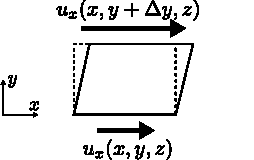
\includegraphics{aero/img/shear.pdf}
  \caption{$x$--$y$平面における速度差 .}
  \label{fig:shear}
\end{figure}
このとき,速度差に比例したせん断応力
\footnote{せん断応力とは,ある面に対して平行に作用する単位面積あたりの力のことである.}
 (Shear stress) が発生すると考えられる
\footnote{
  これは分子運動論から説明ができる.
  せん断応力とはつまるところ分子の運動量が与える影響であり,相対的に速度が速い側の運動量が遅い側に伝わることで発生するとみることができる.
  より詳細なボルツマン方程式から流体力学を構成するフレームワークとして,Chapman--Enskog理論がある.
  % 概要は \url{https://en.wikipedia.org/wiki/Chapman%e2%80%93Enskog_theory} (Accessed on 2025/8/31) を参照されたい.
}.
\begin{equation*}
  F_{xy} \propto \frac{u_x(x, y + \Delta y, z) - u_x(x, y, z)}{\Delta y} \approx \frac{\partial u_x}{\partial y}\qquad
  \text{i.e.}\quad  F_{xy} = \mu \frac{\partial u_x}{\partial y}
\end{equation*}
この比例定数 $\mu$ を \keyword{粘性率} という.
また,$F_{xy}$というのは,法線方向が$y$軸方向の面について$x$軸方向に作用するせん断応力という意である.

ところで,剛体の要素の位置関係が変わらない運動として,平行移動の他に全体が一様に回転する剛体回転がある.
そこで,回転する流速場として$\mathbf{u}(x, y, z) = (-\Omega y, \Omega x, 0)$を考えてみよう.
これは図を書けば明らかなように,全体が一様に回転する流れであり,個々の要素の位置関係は変わらないためせん断応力は$0$になる.
この速度場を先の式に代入してみると,せん断応力が生じてしまうことが分かる.
そこで,このような剛体回転においてはせん断応力が生じないように,以下のように修正しよう.
\begin{equation*}
  F_{xy} = \mu \left(\frac{\partial u_x}{\partial y} + \frac{\partial u_y}{\partial x}\right)
\end{equation*}
これにより,剛体回転においてもせん断応力が$0$になるように修正される.

流体は等方的であることが期待されるから,任意の方向に対して同様の関係が成り立つと考えられる.

\begin{definition}{ニュートンの粘性法則}{}{}
  ニュートンの粘性法則とは,流体のせん断応力がその速度勾配に比例することを示す法則である.
  \begin{equation*}
    \tau \propto \left( \frac{\partial u}{\partial y} \right)
  \end{equation*}


\end{definition}


\subsection{ベルヌーイの定理}

\subsection{境界方程式とレイノルズ数}

\section{ポテンシャル流}

\chapter{空気力学}

\section{ポテンシャル流と抗力・揚力}
\subsection{抗力とダランベールのパラドクス}

\subsection{循環と揚力}

\section{バロウマン法}
\subsection{法線力}
\subsection{圧力中心}


\section{超音速域での空力}
\subsection{音速とマッハ数}

\subsection{Prandtl--Glauert変換}

\subsection{窒息流}


\chapter{数値解析}

\section{CFDの基礎}
\subsection{解析手法}

\section{飛行シミュレーションの基礎}
\subsection{運動方程式を立てる}


\appendix

\chapter{数学的補足}
\section{クォータニオン}

\chapter{材料力学の基礎}

\chapter{自作エンジンの基礎}
\section{ハイブリッドエンジンの燃焼理論}
\section{流量係数}
\section{ノズル理論}

% this is a pull request test text

\bibliography{bib/ref}
\bibliographystyle{junsrt}

\end{document}
